\documentclass[11pt]{article}
\usepackage{amsmath}
\usepackage{physics}
\usepackage{amssymb}
\usepackage{graphicx}
\usepackage{hyperref}
\usepackage{amsfonts}
\usepackage{cancel}
\usepackage{xcolor}
\hypersetup{
	colorlinks,
	linkcolor={black!50!black},
	citecolor={blue!50!black},
	urlcolor={blue!80!black}
}
\newcommand{\f}[2]{\frac{#1}{#2}}
\usepackage{newpxtext,newpxmath}
\usepackage[left=1in,right=1in,top=0.9in,bottom=0.9in]{geometry}
\usepackage{framed}
\usepackage{caption}
\usepackage{subcaption}





\begin{document}
\begin{center}
{\large \bf PH312: Physics of Fluids (Prof. McCoy) -- Reflection}\\
{ Huan Q. Bui}\\
Mar 24 2021
\end{center}


I liked the dimensional analysis we did this week and was specifically surprised by how naturally the Reynolds number appears from this argument.  It was also cool to see how the two kinds of drag forces come out of the different flow regimes. I have been aware of these two drag forces since high school, but never really knew where they come from and thought that they were discovered (and justified) only experimentally. So, finally seeing where their origins was very nice. \\




I was also surprised by how long it took for people to resolve the paradoxical nature of the inviscid flow problem. It's even more interesting that the ``boundary layer'' resolution by Prandtl was actually very intuitive and grounded not on mathematical reasoning alone but also on physical intuition (\textcolor{blue}{which is why I like physics more than pure math -- please don't tell my math professors}). What took scientists so long to figure this out?\\


Last thing... even though the inviscid flow theory requires a ``boundary layer'' to make sense when describing normal fluids, I would think that it can describe superfluids [\textit{e.g. supercooled $^4$He, supercooled $^3$He, Bose-Einstein condensates of fermion pairs (i.e. Cooper-pair superfluid), etc.}] to some extent. Obviously there are quantum mechanical effects [\textit{e.g. quantized vortices in a rotating superfluid, density and temperature oscillation (or \textit{first} and \textit{second} sounds), etc.}], but I wonder how many properties of superfluidity the Euler equation can predict. \\


Attached is what happens when you stir a $^6$Li fermionic superfluid using a laser. Instead of having bulk rotation (like when stirring water in a cup), quantized vortices are formed. This is a quantum mechanical effect predicted by Lars Onsager in 1949 (it has to do with the superfluid having a macroscopic wavefunction, which has a phase, which quantizes circulation).

\begin{figure}[!htb]
	\centering
	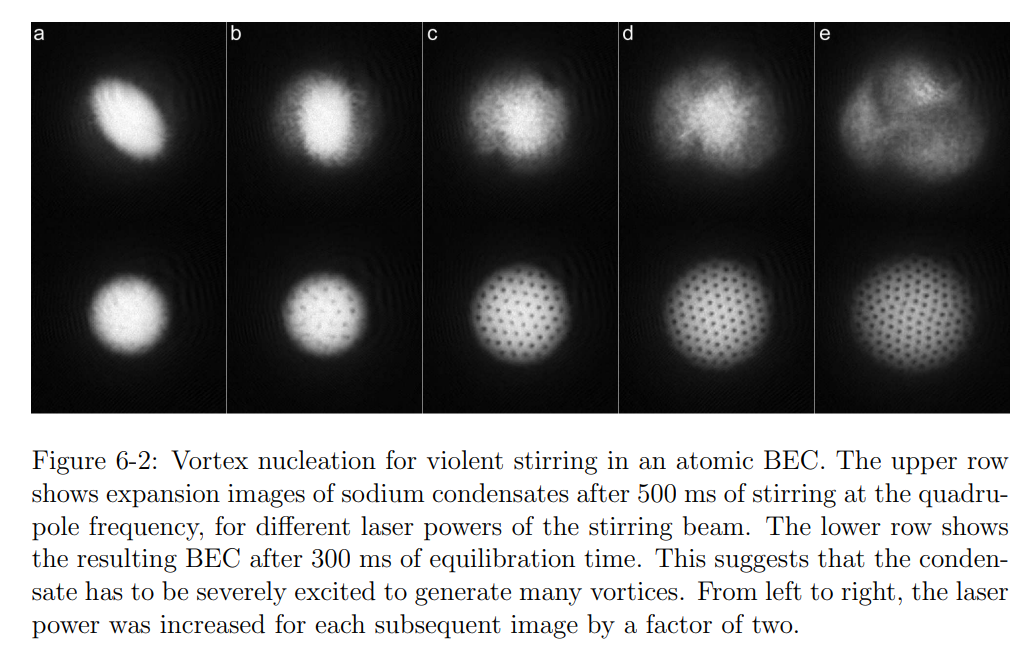
\includegraphics[scale=0.4]{BEC_vortex}
\end{figure}

This image was taken from Martin Zwierlein's \href{https://www.rle.mit.edu/cua_pub/ketterle_group/Theses/Zwierlein_Thesis_Adobe7.pdf}{\underline{\texttt{PhD Thesis}}} under Wolfgang Ketterle at MIT. You can also read about this in \href{https://www.nature.com/articles/nature03858}{\underline{\texttt{Nature}}}. I actually don't just randomly know about and become interested in this work. I do because I will be starting my PhD in Prof. Zwierlein's group at MIT this summer (working on newer but related projects, of course)! :) 












  
\end{document}




